\chapter{Analisi del Layout PCB}

Una volta terminato il progetto dello schematico e verificata la sua
correttezza, siamo passati allo sbroglio circuitale. Abbiamo quindi
esportato la netlist da \emph{eeschema} per poi importarla in
\emph{pcbnew}, popolando il progetto con i footprint di tutti i
componenti.

\hypertarget{layout}{%
\section{Layout}\label{layout}}

Come primo passo abbiamo raggruppato i vari componenti per sezione
circuitale (alimentazione, microcontrollore, controllo motori,
ecc\ldots) in modo da avere un primo ordine.\\
Fino a questo punto non abbiamo posto alcun riguardo verso la posizione
dei componenti, ma abbiamo semplicemente effettuato una suddivisione
funzionale. Con il passo successivo abbiamo invece collocato, per
ciascun blocco circuitale, ogni componente nel modo che più ci è
sembrato adeguato, tenendo in mente gli aspetti elettrici (per esempio
il posizionamento del GPS lontano dalla sezione di potenza e dal
microcontrollore), di distanziamento, di funzionalità (per esempio
posizionamento di connettori e pulsanti), di comodità per l'utente
finale ed infine di estetica.\\
Per quanto riguarda la sezione legata al microcontrollore abbiamo
posizionato, in ordine di priorità:

\begin{enumerate}
\def\labelenumi{\arabic{enumi}.}
\item
  
  il quarzo con i suoi condensatori ed il suo resistore il più vicino
  possibile ai pin \textit{XIN} e \textit{XOUT};
  
\item
  
  i condensatori di decoupling più vicini possibile ai pin di
  alimentazione;
  
\item
  
  la memoria flash;
  
\item
  
  i resistori di terminazione della linea USB.
  
\end{enumerate}

\begin{center}
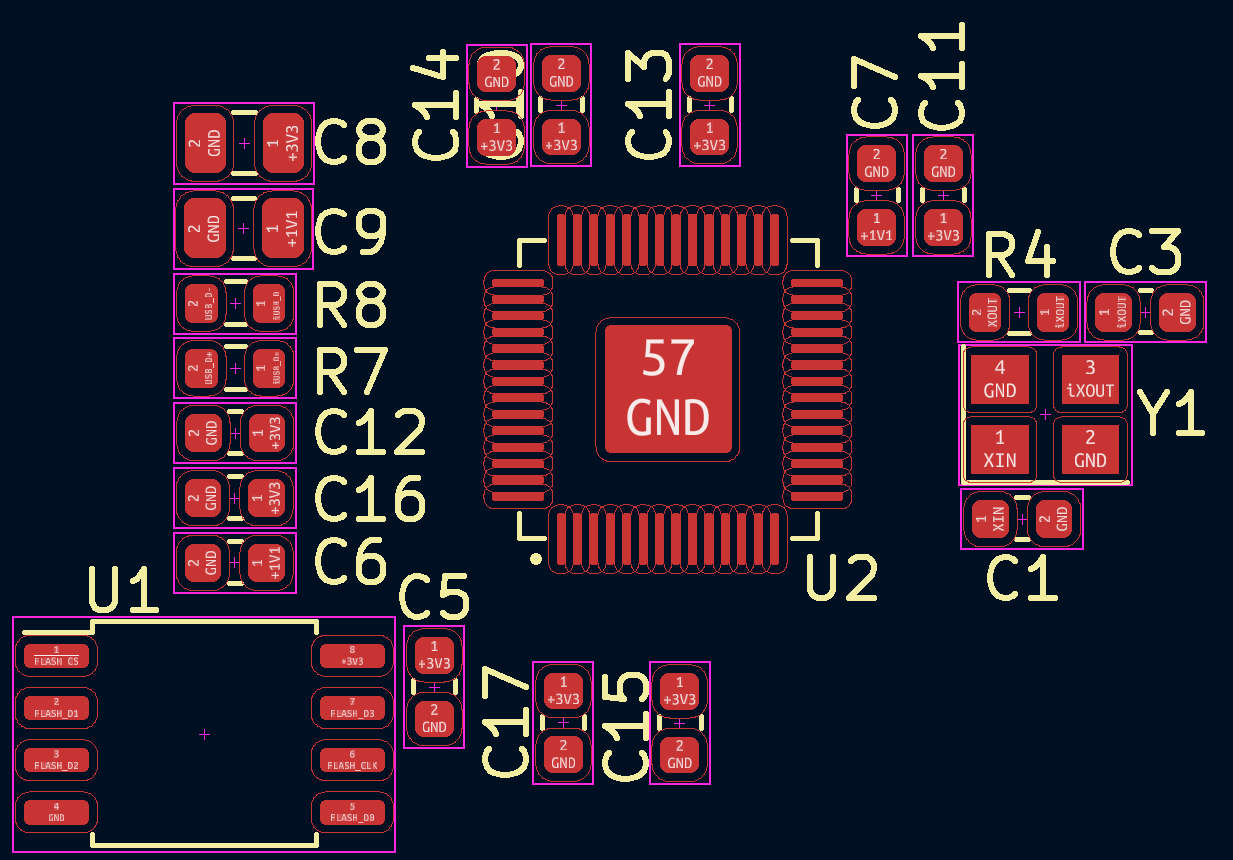
\includegraphics[scale=0.3]{figures/image29.png}
\captionsetup{type=figure}
\captionof{figure}{Primo posizionamento componenti principali foglio Control}
\end{center}

\noindent Il fatto di posizionare i componenti il più vicino possibile ai relativi
pin è necessario per ridurre di quanto possibile l'impedenza della linea
di alimentazione, e quindi la lunghezza del percorso del segnale.
Maggiore è la lunghezza del percorso tra condensatore e pin e maggiore
sarà l'induttanza parassita della traccia, che porta a problemi di
integrità di segnale quando si ha a che fare con segnali ad alta velocità.
Considerando a titolo di esempio una linea di alimentazione,
l'induttanza parassita è contrastata dalla presenza dei condensatori di
decoupling. In questo modo siamo in grado fornire un percorso a bassa
impedenza tra condensatore e pin del MCU, perciò la restante lunghezza
che va dal condensatore al pin di alimentazione deve rimanere il più
breve possibile. Si noti che ai fini del calcolo si deve considerare sia
la linea di andata (es: alimentazione) che quella di ritorno (GND).\\
Per quanto riguarda la sezione di controllo dei motori abbiamo
posizionato i connettori, i transistor, i diodi ed i resistori di
polarizzazione in modo da ridurre al minimo le tracce necessarie e da
allineare il tutto per renderlo il più esteticamente bello possibile.

\begin{center}
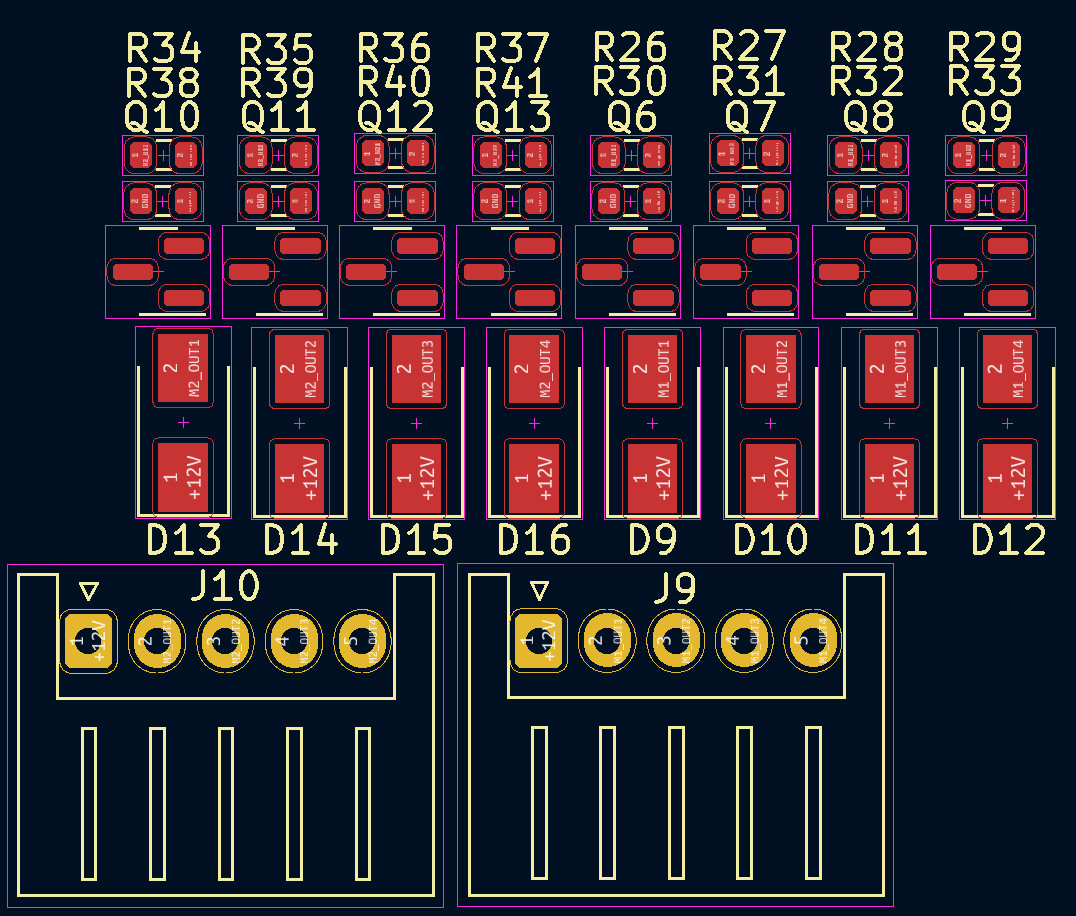
\includegraphics[scale=0.3]{figures/image55.png}
\captionsetup{type=figure}
\captionof{figure}{Primo posizionamento componenti driver motori stepper}
\end{center}

\noindent Parlando dello stadio di alimentazione, abbiamo posizionato tutti i
componenti in modo da minimizzare il numero di tracce necessarie e da
facilitare il routing di tracce di grande spessore. Abbiamo rivolto
particolare attenzione al regolatore a commutazione, cercando di rendere
il nodo di switching più piccolo possibile per ridurre al minimo il
\textit{ripple}.

\begin{center}
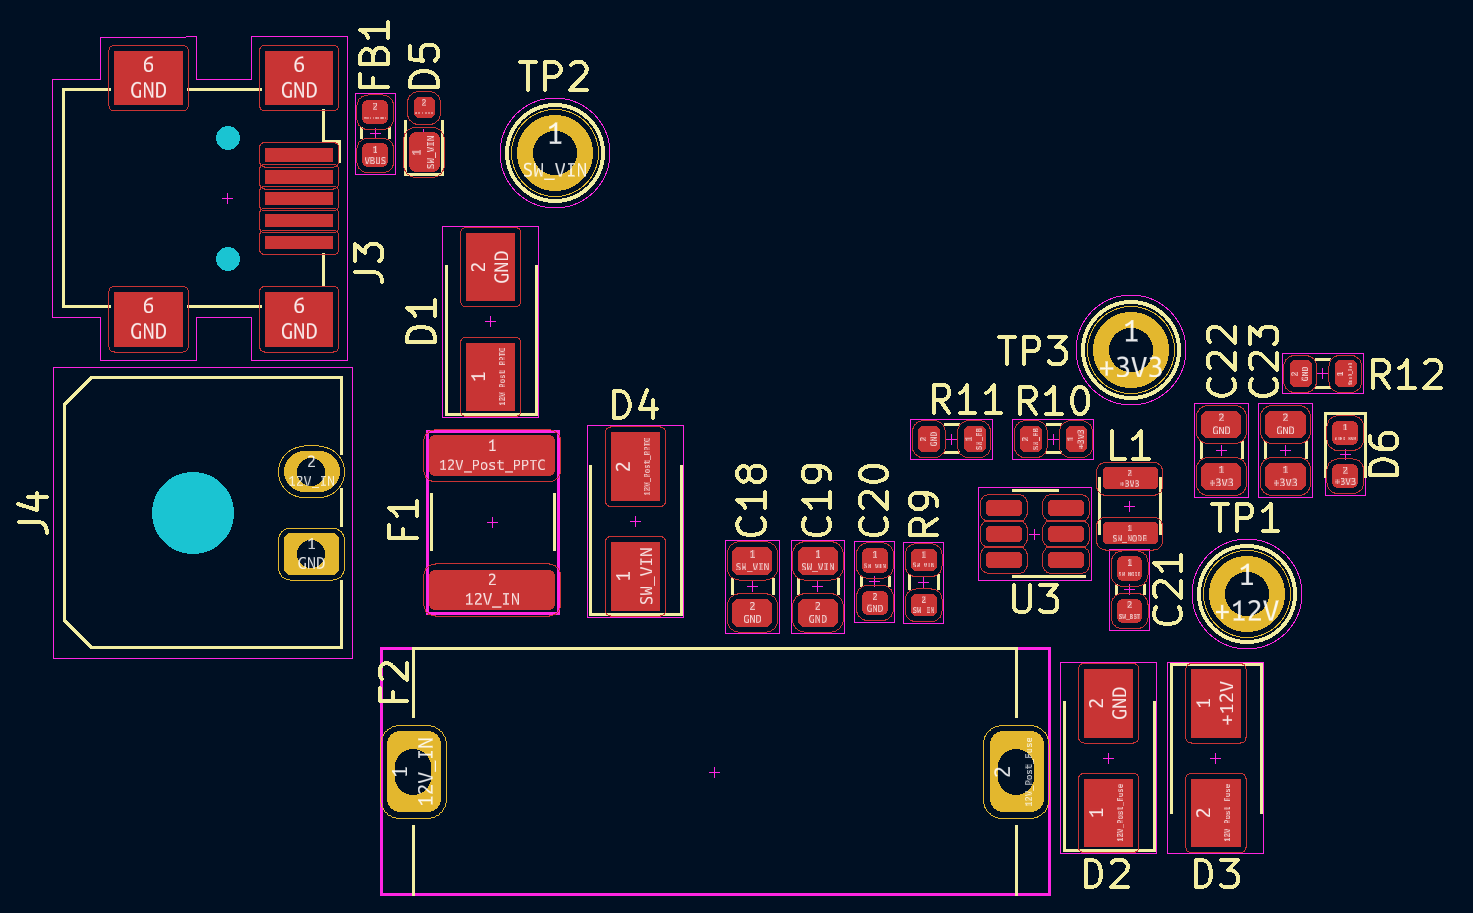
\includegraphics[width=0.5\textwidth]{figures/image56.png}
\captionsetup{type=figure}
\captionof{figure}{Primo posizionamento componenti foglio Power}
\end{center}

\noindent Le restanti sezioni non includono componenti particolarmente critici,
quindi il posizionamento è stato fatto seguendo il principio di
semplicità di routing delle tracce e di bellezza estetica.\\
A questo punto, dopo aver ottenuto un insieme di diversi blocchi
circuitali, abbiamo provato a posizionarli in modo da capire che
dimensioni imporci come limite per la scheda ed abbiamo appurato che
100x60mm fosse una misura adeguata per contenere il tutto.\\
Avendo definito le dimensioni siamo passati alla creazione del disegno
del contorno della scheda sul layer \textit{Edge.Cuts}, introducendo un
arrotondamento degli angoli per fini puramente estetici. Successivamente
abbiamo disegnato i rettangoli di riempimento, assegnandoli alla net di
GND e con priorità minima per entrambi i layer, in modo che coprissero
la scheda intera.\\
Abbiamo quindi posizionato i blocchi circuitali discussi in precedenza,
non prima di aver posizionato i fori di montaggio ed i \textit{fiducials},
facendo in modo di avere i connettori lungo il bordo. Anche il \textit{GPS} è
stato posizionato in un angolo in modo da tenerlo il più lontano
possibile da ogni altro componente; sotto il suo ingombro abbiamo
inserito anche una \emph{keepout zone}, come richiesto da datasheet.

\begin{center}
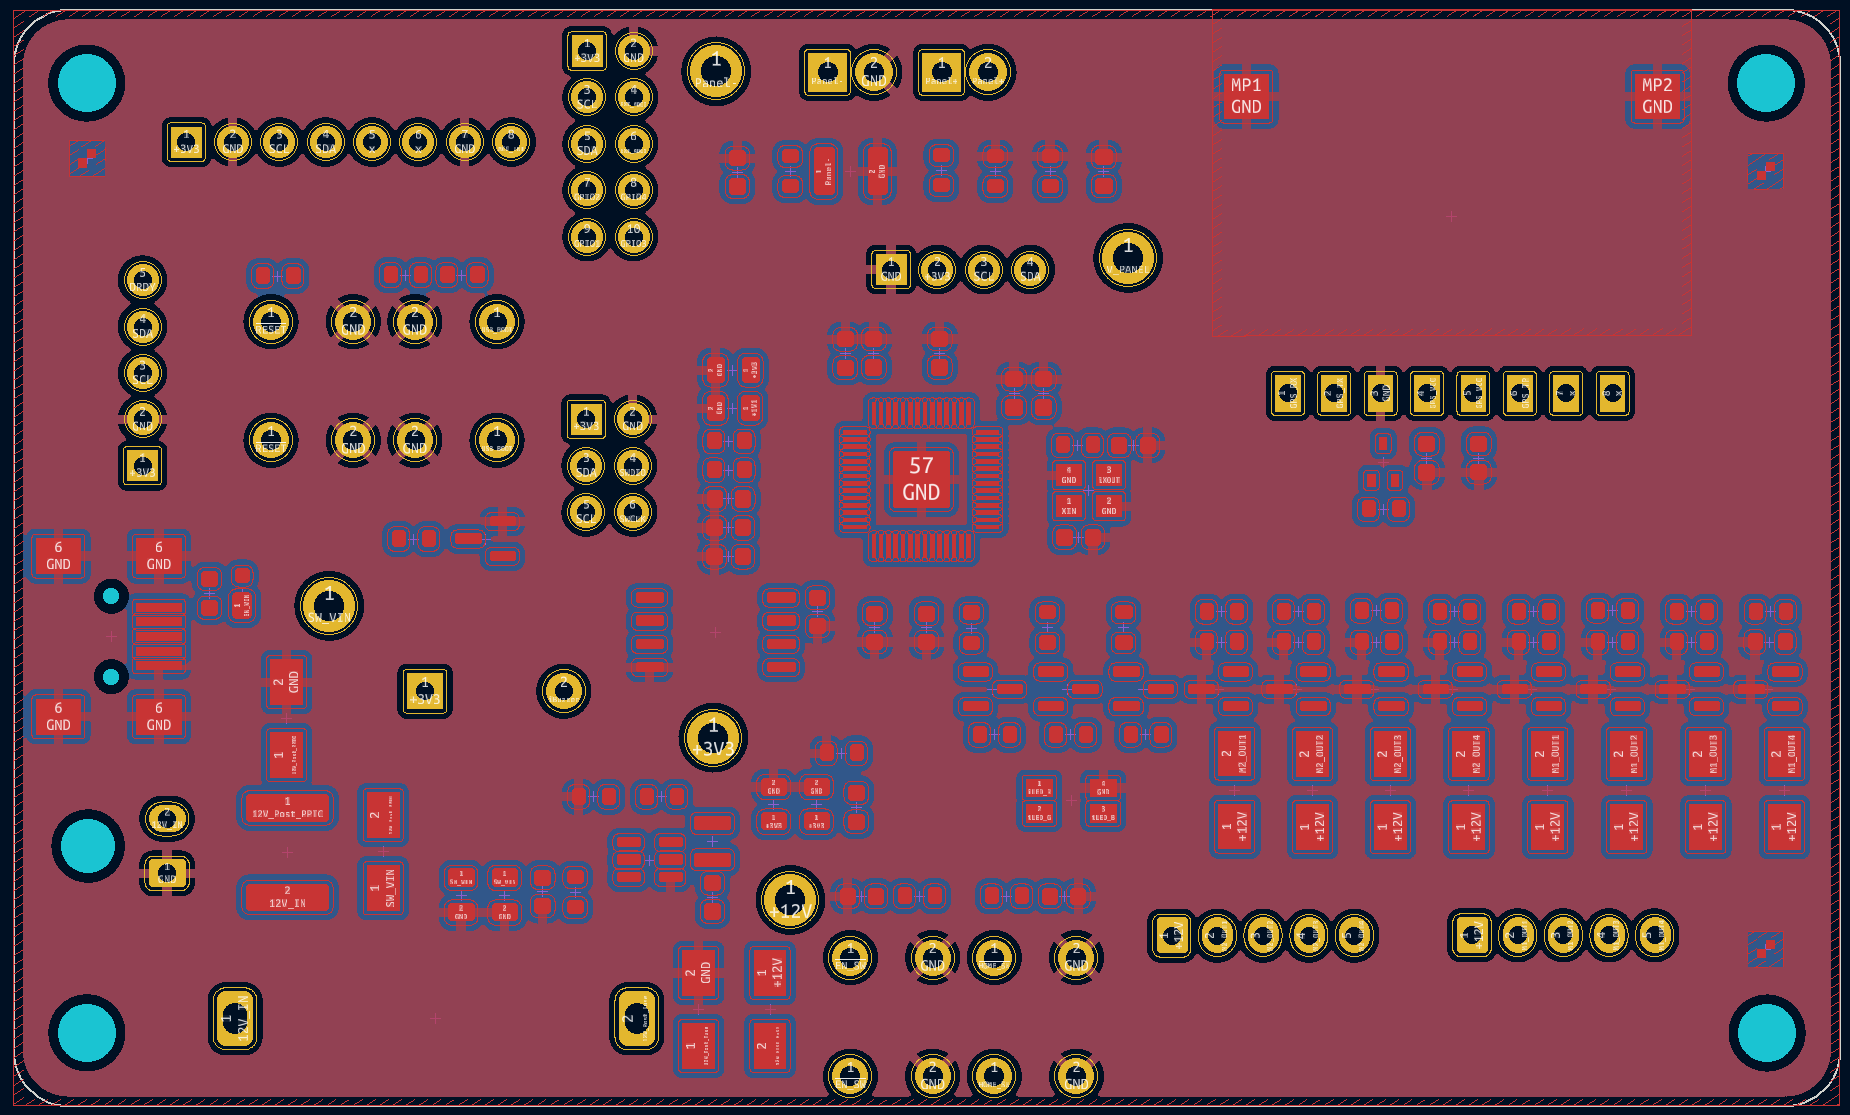
\includegraphics[width=4.57535in,height=2.75694in]{figures/image21.png}
\captionsetup{type=figure}
\captionof{figure}{Prima bozza piazzamento componenti}
\end{center}

\hypertarget{routing}{%
\section{Routing}\label{routing}}

\noindent Una volta definite le posizioni dei vari componenti siamo passati alla
fase di routing, cominciando dalle linee particolarmente sensibili e poi
quelle di alimentazione. Prima di iniziare abbiamo creato una serie di
dimensioni predefinite per le tracce:

\begin{itemize}
\item
  
  0.2mm per il \textit{fanout} del microcontrollore
  
\item
  
  0.3mm per le linee di segnale in generale
  
\item
  
  0.5mm per le linee di alimentazione
  
\item
  
  0.8mm per le linee di alimentazione dei motori
  
\end{itemize}

\noindent Abbiamo inoltre creato due dimensioni predefinite per le \textit{vias} (diametro
pad/diametro foro):

\begin{itemize}
\item
  
  0.55mm/0.25mm per le linee di segnale
  
\item
  
  0.8mm/0.4mm per le linee di alimentazione
  
\end{itemize}

\noindent Una volta preparato l'ambiente di lavoro abbiamo cominciato a collegare
tutte le linee di alimentazione, partendo prima da quelle più corte che,
per esempio, collegano un pin di un dispositivo al relativo condensatore
di decoupling, per effettuare solo alla fine i collegamenti più lunghi
facendo in modo di lasciare sufficiente spazio per le linee di segnale.\\
Per quanto riguarda il routing dell'alimentazione vogliamo sottolineare
3 accorgimenti che abbiamo preso:

\begin{itemize}
\item
  
  per le tracce che vanno dal connettore del pannello solare allo shunt
  per misurare la corrente, abbiamo deciso di utilizzare uno spessore di
  1mm, in modo da ridurne al minimo la resistenza;
  
\item
  
  per effettuare il fanout del microcontrollore abbiamo utilizzato
  tracce da 0.2mm per allontanarsi dai pin, per poi allargarle il prima
  possibile a 0.3mm;
  
\item
  
  per il routing della linea di alimentazione a 12V per il controllo dei
  motori abbiamo utilizzato per quanto possibile i poligoni di
  riempimento, assegnando la net 12V ed impostando la priorità ad 1.
  
\end{itemize}

\begin{center}
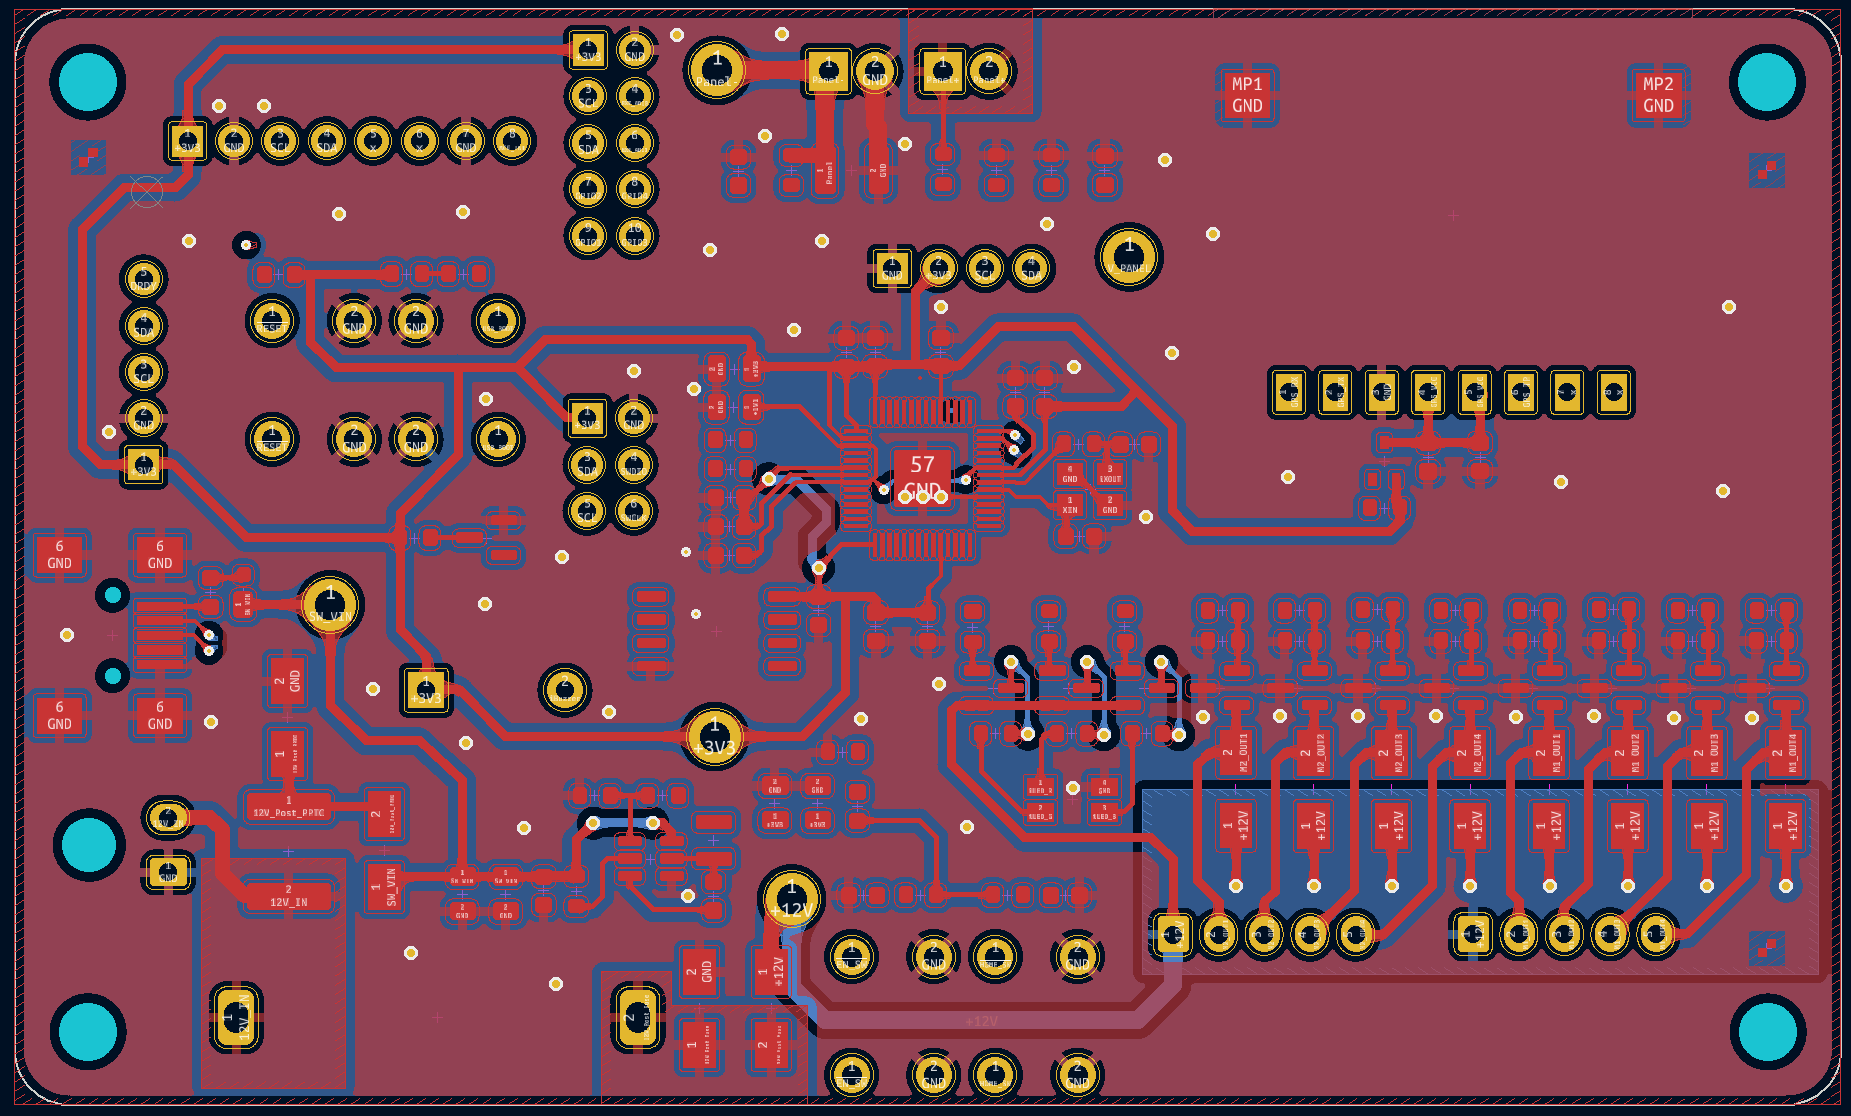
\includegraphics[scale=0.2]{figures/image77.png}
\captionsetup{type=figure}
\captionof{figure}{Prima bozza routing tracce}
\end{center}

\noindent Una volta concluso il routing delle linee di alimentazione siamo passati
alle restanti linee di segnale iniziando dal fanout del
microcontrollore, anche in questo caso partendo con tracce da 0.2mm per
poi allargarle a 0.3mm.\\
Abbiamo considerato per primi i segnali critici, ovvero le linee del
quarzo, quelle per la trasmissione \textit{QSPI} della flash e quelle
differenziali per l'USB. Sebbene non sia di apprezzabile effetto dal
punto di vista funzionale, abbiamo voluto provare, a titolo di esercizio
personale, il tool di \emph{length matching} per rendere le linee
differenziali D+ e D- dell'USB più simili possibile in termini di
lunghezza. Questo è stato fatto, perché abbiamo riscontrato alcune
difficoltà nell'utilizzo del router differenziale, che avrebbe gestito
il \emph{length matching} in autonomia.\\
Avendo definito le tracce critiche siamo poi passati al fanout e al
routing dei restanti segnali. Durante questo processo abbiamo iterato
più volte spostando le assegnazioni di alcuni pin del microcontrollore,
grazie alle matrici di assegnazione dei GPIO, in modo da trovare le
posizioni ottimali.\\
Questa parte dello sbroglio è stata la più complessa a causa della
necessità di avere molti dispositivi vicini al microcontrollore e alla
ridotta \emph{clearance} tra i pin.

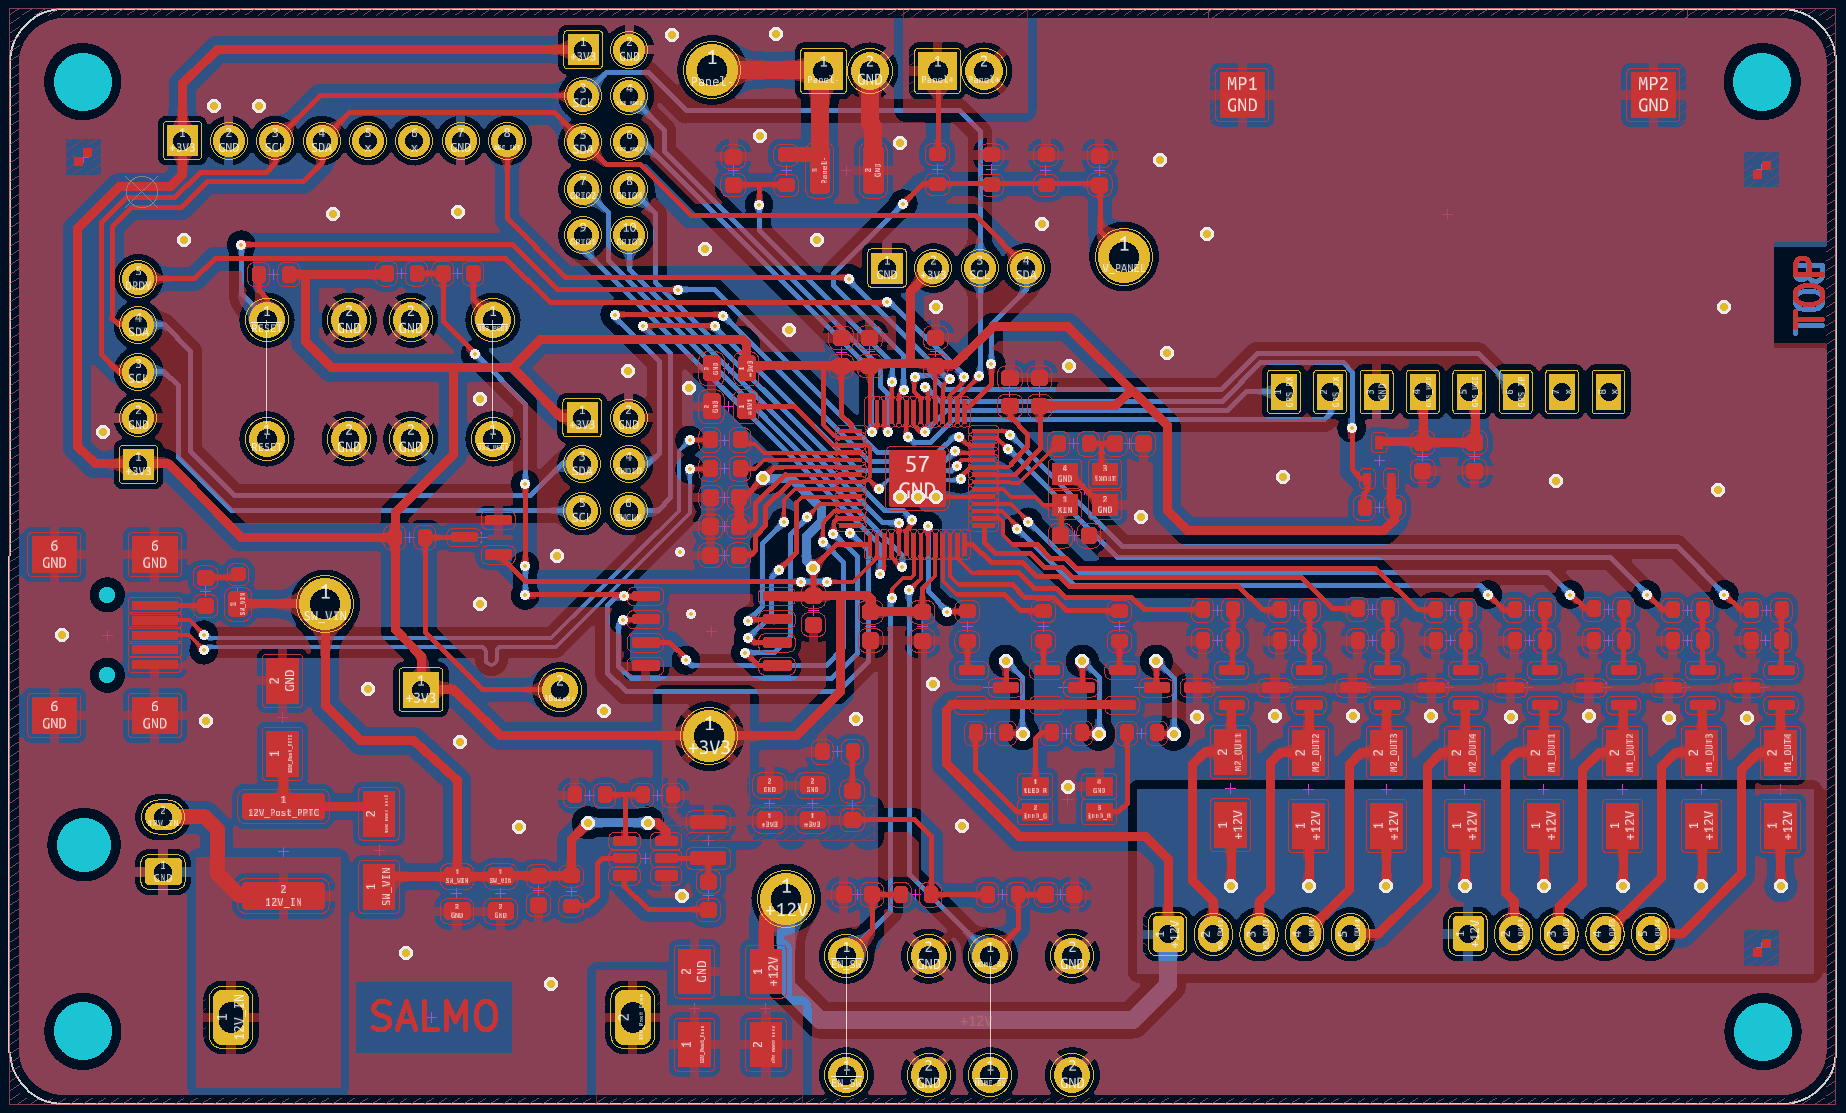
\includegraphics[scale=0.16]{figures/image59.png}
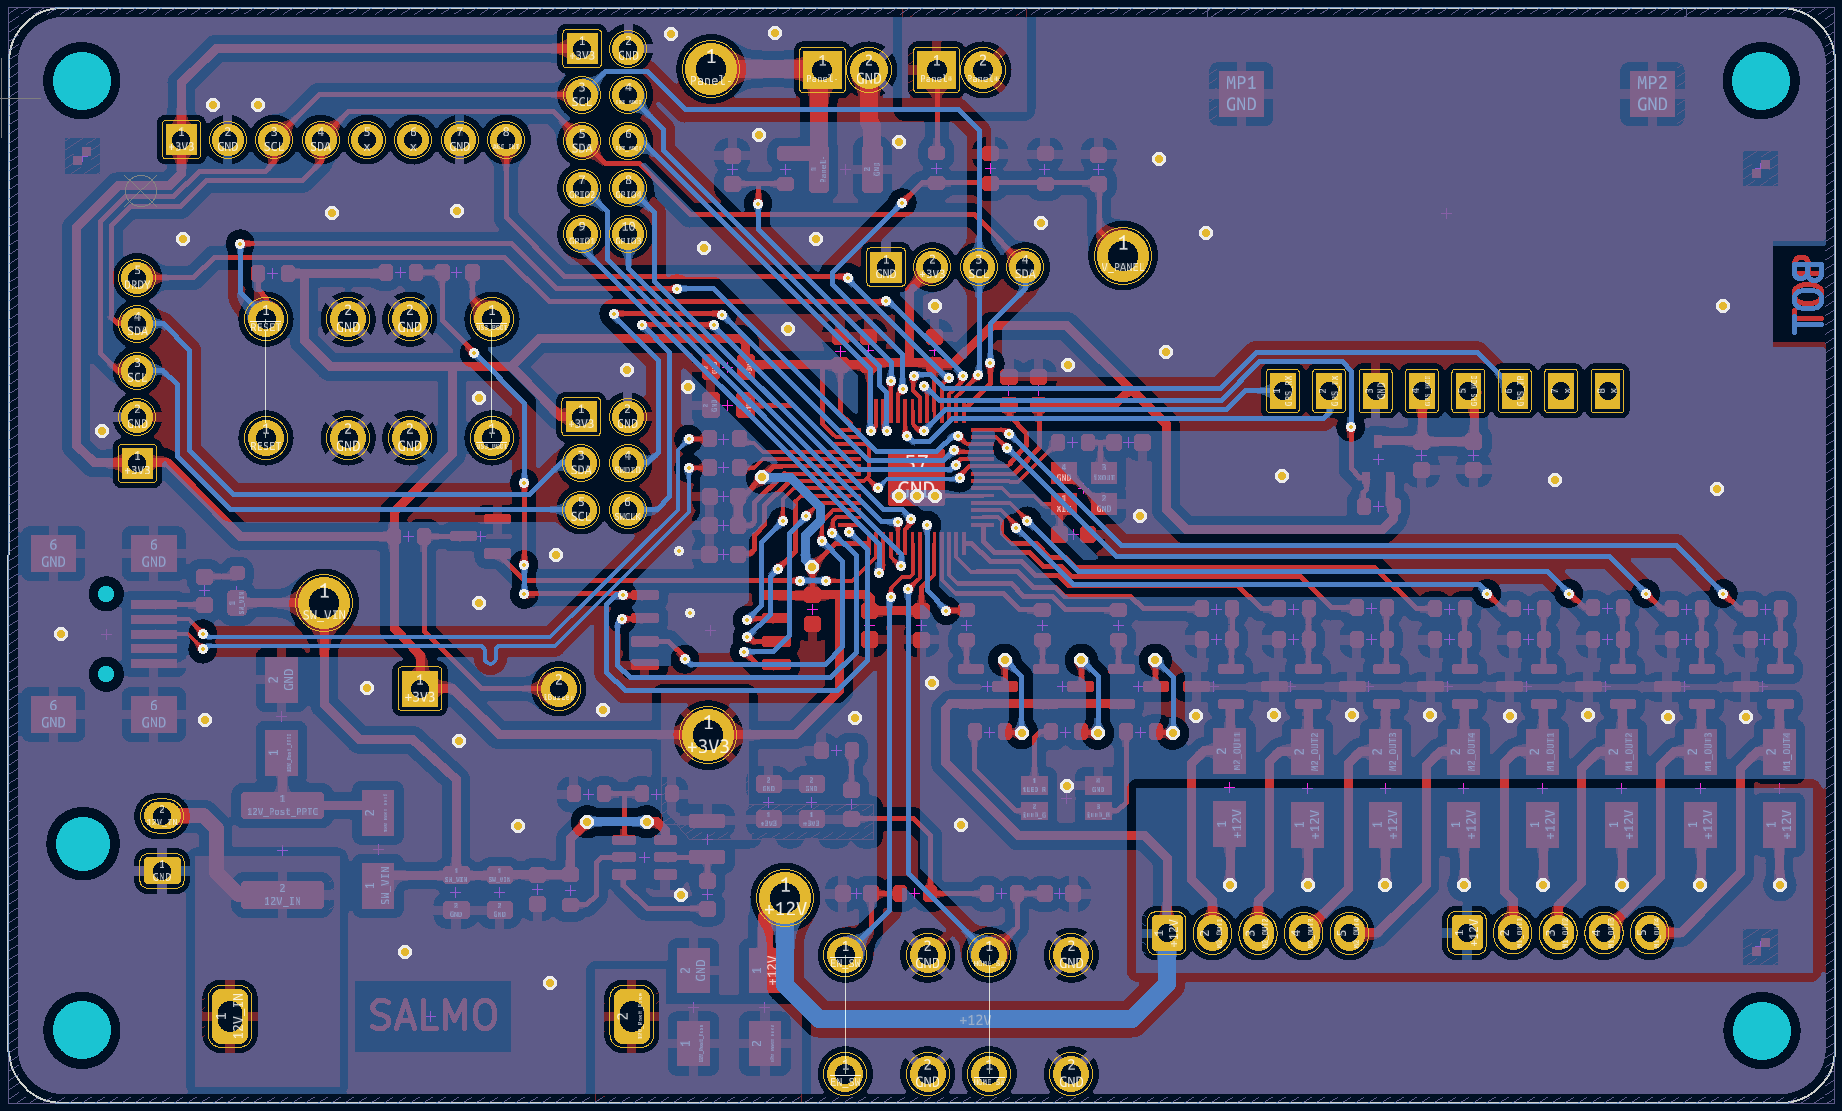
\includegraphics[scale=0.16]{figures/image22.png}
\begin{center}
\captionsetup{type=figure}
\captionof{figure}{Primo risultato routing PCB}
\end{center}

\noindent Terminato il routing di tutte le tracce abbiamo fatto un'analisi per
cercare eventuali sviste o errori commessi, sia facendo un'ispezione
visiva, sia utilizzando il \textit{DRC}. Prevedibilmente abbiamo riscontrato
qualche errore che abbiamo prontamente corretto senza troppe difficoltà.\\
Anche dopo queste correzioni il \textit{DRC} restituisce alcuni errori, che però
sono previsti e non causano problemi nella realizzazione. Questi sono di
due tipi, il primo è il \emph{Courtyards overlap} per i componenti che
stanno vicino al \textit{GPS}, mentre il secondo è l' \emph{Items not allowed} ed
è dovuto a come sono stati realizzati i footprint dei fiducials.\\
Il primo lo si può ignorare, perché in realtà il \textit{GPS} sarà montato su un
header rialzato e quindi la superficie del PCB sarà libera da
occlusioni. Il secondo errore invece è dovuto al fatto che il footprint
dei \textit{fiducials} è stato realizzato con due pad che sovrappongono una
\emph{keepout zone}, questo però è comunque un effetto desiderato,
quindi possiamo ignorarlo.

\hypertarget{finitura}{%
\section{Finitura}\label{finitura}}

\noindent Arrivati a questo punto abbiamo appurato che l'aspetto elettrico della
scheda era corretto, quindi ci siamo concentrati sugli aspetti estetico
e utilitario.\\
Prima di tutto abbiamo aggiunto un pad di GND a lato scheda per poter
collegare una pinza a coccodrillo in modo da semplificare le misurazioni
per il debug hardware. Poi abbiamo fatto in modo di posizionare, sul
layer \textit{silkscreen} tutti i \textit{refdes} dei componenti, in modo tale che fossero
ordinati e ben visibili, facendo particolare attenzione, per quanto
possibile, a non posizionarli sopra vias che avrebbero causato
potenziali problemi di lettura.

\begin{center}
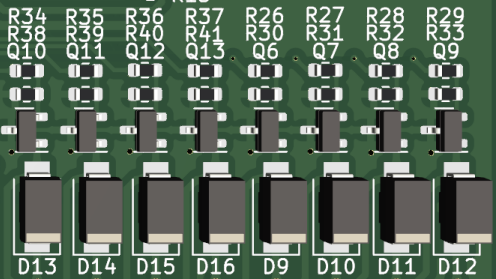
\includegraphics[width=0.5\textwidth]{figures/image100.png}
\captionsetup{type=figure}
\captionof{figure}{Esempio Silkscreen SALMO}
\end{center}

\noindent Sistemati tutti i \textit{refdes} abbiamo aggiunto sui layer di \textit{silkscreen}
ulteriori descrizioni per chiarire le funzioni dei connettori e per
aggiungere informazioni utili. In particolare abbiamo aggiunto 
l’indicazione di polarità sul connettore di alimentazione e, ad ogni
connettore il suo nome e, sul retro, la descrizione di ogni pin. Per i
connettori di espansione e debug non c'era spazio a sufficienza, quindi
abbiamo creato sul retro una grafica apposita composta da una tabella,
che rappresenta la funzione di ogni pin, e da un segmento di retta che
riconduce la tabella al connettore a cui fa riferimento.\\
Abbiamo successivamente aggiunto, sempre sul retro, il titolo del
progetto con il nome del corso, nomi, cognomi e matricole dei membri del
gruppo e data e numero di revisione.

\begin{center}
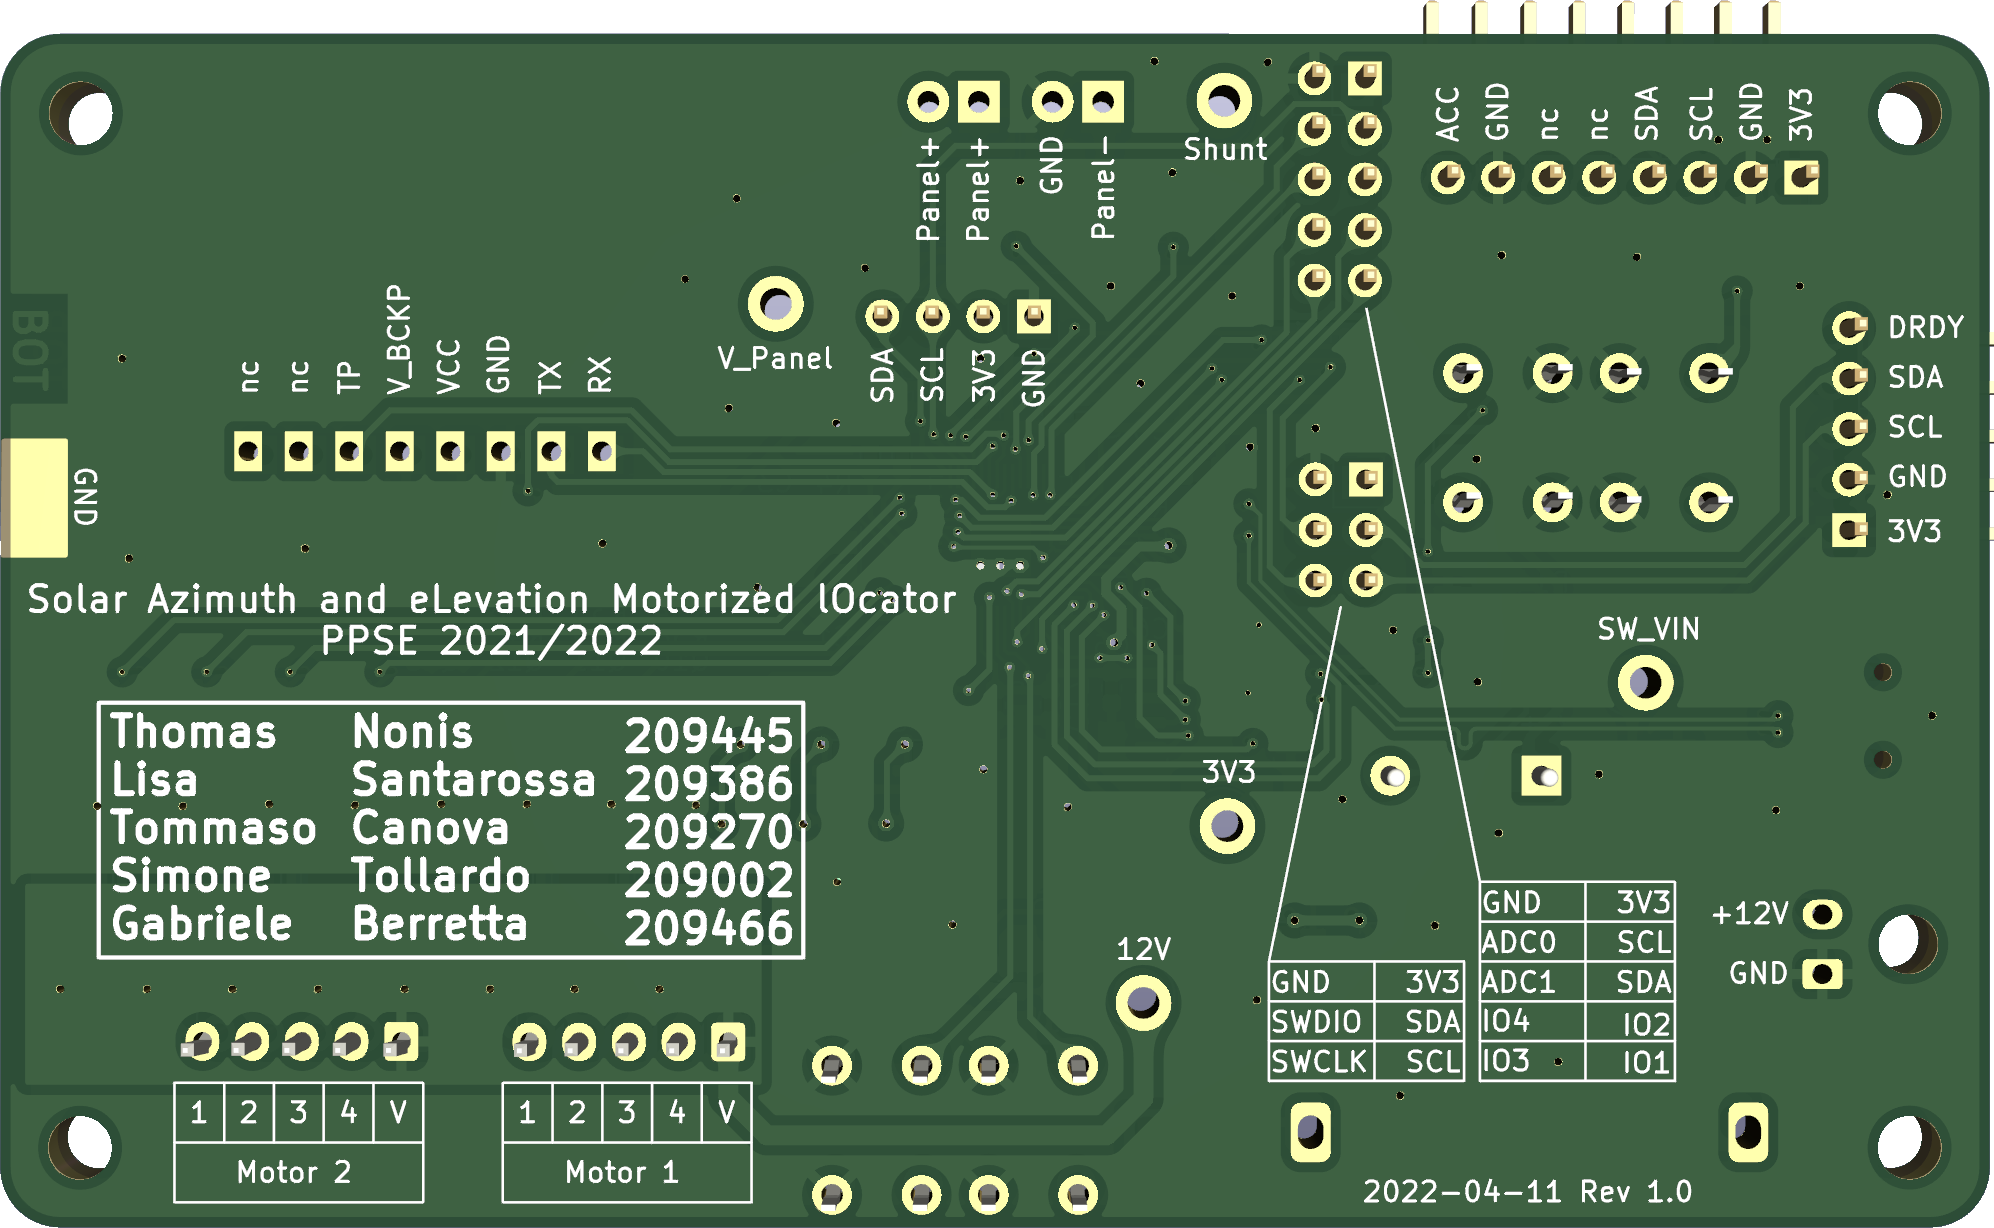
\includegraphics[scale=0.2]{figures/image42.png}
\captionsetup{type=figure}
\captionof{figure}{Vista del retro della PCB SALMO}
\end{center}

\noindent Per poter facilmente identificare i layer \textit{top} e \textit{bottom} abbiamo aggiunto,
a lato scheda, i testi TOP e BOT sui layer corrispondenti.\\
A questo punto la scheda si può considerare terminata e non è rimasto
altro da fare che generare i \textit{teardrops}, tramite un plugin dedicato, ed
esportare i file \textit{gerber} e \textit{drill} (che riportiamo negli allegati della
presente relazione).\\
A questo punto abbiamo importato i file \textit{gerber} in \emph{gerbview} per un
controllo finale. Grazie a quest'ultima ispezione abbiamo identificato
qualche piccolo errore che abbiamo prontamente corretto. Abbiamo infine
mandato tutti i file al Professore, che ha provveduto all'invio di
questi al produttore.
